
 % Preamble: \usepackage{graphicx,array}
\setlength{\tabcolsep}{0.5pt}
\renewcommand{\arraystretch}{1.0}

\begin{figure}[t]
\centering
\newcommand{\imgw}{0.24\linewidth} % 4 images × 0.24 = 0.96 (safe)
\begin{tabular}{@{}cccc@{}}
  % Header
  % \multicolumn{4}{@{}l@{}}{{\scriptsize\textbf{Structured edits (disentanglement)}}} \\[-1pt]

  % Images (row)
  % \multicolumn{4}{c}{\textit{``A mother duck guards three rubber duckies.''}} \\
  % \multicolumn{4}{c}{\textit{``A bouquet of  flowers is upside down in a vase.''}} \\
  % \includegraphics[width=\imgw]{Figures/contextual_contradictions/images/vase/flux.png} &
  % \includegraphics[width=\imgw]{Figures/contextual_contradictions/images/vase/hidream.jpg} &
  % \includegraphics[width=\imgw]{Figures/contextual_contradictions/images/vase/qwen.jpg} &
  % 
\includegraphics[width=\imgw]{Figures/contextual_contradictions/images/vase/bria_new.jpg}
  % \\[-2pt]

    % Images (row)
      \multicolumn{4}{c}{\textit{``A bear is performing a
handstand in the park.''}} \\
  \includegraphics[width=\imgw]{Figures/contextual_contradictions/images/bear/flux.png} &
  \includegraphics[width=\imgw]{Figures/contextual_contradictions/images/bear/hidream.jpg} &
  \includegraphics[width=\imgw]{Figures/contextual_contradictions/images/bear/qwen.jpg} &
  \includegraphics[width=\imgw]{Figures/contextual_contradictions/images/bear/bria_new_new.jpg}
  \\%[-2pt]

    % Images (row)

    \multicolumn{4}{c}{\textit{``A woman writing with a dart.''}} \\
  \includegraphics[width=\imgw]{Figures/contextual_contradictions/images/woman_dart/flux.png} &
  \includegraphics[width=\imgw]{Figures/contextual_contradictions/images/woman_dart/hidream.jpg} &
  \includegraphics[width=\imgw]{Figures/contextual_contradictions/images/woman_dart/qwen.jpg} &
  \includegraphics[width=\imgw]{Figures/contextual_contradictions/images/woman_dart/bria_new_new.jpg}
  \\%[-2pt]
  
  %  \multicolumn{4}{c}{\textit{``A balloon is lifting up a package.''}} \\
  % \includegraphics[width=\imgw]{Figures/contextual_contradictions/images/ballon/flux.jpg} &
  % \includegraphics[width=\imgw]{Figures/contextual_contradictions/images/ballon/hidream.jpg} &
  % \includegraphics[width=\imgw]{Figures/contextual_contradictions/images/ballon/qwen.jpg} &
  % 
\includegraphics[width=\imgw]{Figures/contextual_contradictions/images/ballon/bria_new.jpeg}

  % \\%[-2pt]

% \multicolumn{4}{c}{\textit{``A butterfly is in a bee’s hive.''}} \\
%   \includegraphics[width=\imgw]{Figures/contextual_contradictions/images/butterfly_hive/flux.jpg} &
%   \includegraphics[width=\imgw]{Figures/contextual_contradictions/images/butterfly_hive/hidream.jpg} &
%   \includegraphics[width=\imgw]{Figures/contextual_contradictions/images/butterfly_hive/qwen.jpg} &
%   \includegraphics[width=\imgw]{Figures/contextual_contradictions/images/butterfly_hive/bria_new_3.jpg}

%   \\%[-2pt]

\multicolumn{4}{c}{\textit{``A professional boxer does a split.''}} \\
  \includegraphics[width=\imgw]{Figures/contextual_contradictions/images/boxer/flux.jpg} &
  \includegraphics[width=\imgw]{Figures/contextual_contradictions/images/boxer/hidream.jpg} &
  \includegraphics[width=\imgw]{Figures/contextual_contradictions/images/boxer/qwen.jpg} &
  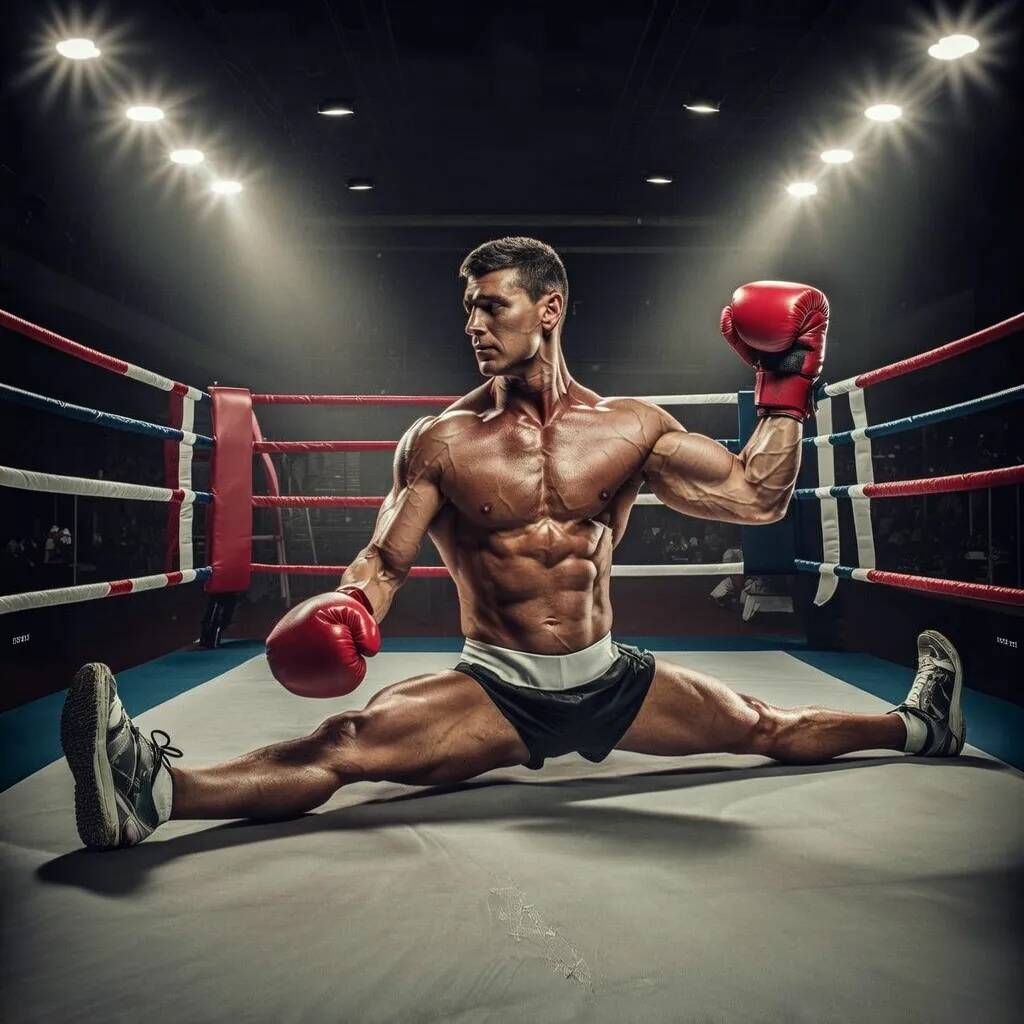
\includegraphics[width=\imgw]{Figures/contextual_contradictions/images/boxer/bria_new.jpeg}

  \\%[-2pt]


  % Wrapped labels under each image (row)
  \parbox{\imgw}{\scriptsize\centering \textbf{FLUX}} &
  \parbox{\imgw}{\scriptsize\centering \textbf{HiDream}} &
  \parbox{\imgw}{\scriptsize\centering \textbf{Qwen-Image}} &
  \parbox{\imgw}{\scriptsize\centering \textbf{Fibo (Ours)}}
  \\
\end{tabular}

\vspace{-3pt}
\caption{\textbf{Contextual contradiction.} We use prompts from ContraBench~\cite{huberman2025image} and Whoops~\cite{Bitton_Guetta_2023}. \modelname{} generates semantically consistent images that faithfully represent the correct relations, unlike other models that often default to typical co-occurrences. }
\label{fig:contextual}
\end{figure}
% Preamble: \usepackage{graphicx,array}
\setlength{\tabcolsep}{0.5pt}
\renewcommand{\arraystretch}{1.0}

\begin{figure}[t]
\centering
\newcommand{\imgw}{0.24\linewidth} % 4 images × 0.24 = 0.96 (safe)
\begin{tabular}{@{}cccc@{}}


\multicolumn{2}{c}{\footnotesize\textit{``Shallow depth of field''}} &
\multicolumn{2}{c}{\footnotesize\textit{``Deep depth of field''}} \\
  \includegraphics[width=\imgw]{Figures/control/flux_shallow.jpg} &
  \includegraphics[width=\imgw]{Figures/control/shallow.jpg} &
  \includegraphics[width=\imgw]{Figures/control/flux_deep.jpg} &
  \includegraphics[width=\imgw]{Figures/control/deep.jpg}

  \\%[-2pt]


  % Wrapped labels under each image (row)
  \parbox{\imgw}{\scriptsize\centering \textbf{FLUX}} &
  \parbox{\imgw}{\scriptsize\centering \textbf{\modelname{} (Ours)}} &
  \parbox{\imgw}{\scriptsize\centering \textbf{Flux}} &
  \parbox{\imgw}{\scriptsize\centering \textbf{\modelname{} (Ours)}}
  \\
\end{tabular}
%\vspace{6pt}

% ---------- Added two-column image table (mirrors style) ----------
\newcommand{\imgwB}{0.48\linewidth} % 2 images × 0.48 = 0.96 (safe)
\begin{tabular}{@{}cc@{}}
\multicolumn{2}{>{\centering\arraybackslash}p{0.96\linewidth}}{%
  \footnotesize\textit{``Three people: Left one holding a goose while screaming. Middle is deeply surprised. Third is crying while holding two piglets.''}%
}\\
\includegraphics[width=\imgwB]{Figures/control/ranch_flux.jpg} &
\includegraphics[width=\imgwB]{Figures/control/ranch_ours.jpg} \\
\parbox{\imgwB}{\scriptsize\centering \textbf{FLUX}} &
\parbox{\imgwB}{\scriptsize\centering \textbf{\modelname{} (Ours)}}
\end{tabular}


\vspace{-3pt}
\caption{\textbf{Controllability examples.} \emph{Top:} Our model (\modelname{}) enables precise depth-of-field control, from shallow to deep, whereas FLUX~\cite{flux2024} does not consistently produce deep depth of field. \emph{Bottom:} \modelname{} allows simultaneous control of facial expressions for multiple subjects within the same scene.}
\label{fig:control}
\end{figure}


\section{Method}
\label{sec:method}

In this section, we present the main contributions of the paper. Section~\ref{sec:captions} introduces the motivation for training with long structured prompts and analyzes their effect on controllability and disentanglement. We also present our workflow, as demonstrated in Figure~\ref{fig:workflow}.
Section~\ref{sec:dimfusion} introduces \emph{DimFusion}, our novel architecture for integrating an LLM with a text-to-image model under reduced computational requirements. 
% This enables us to train with longer, more descriptive captions. %\ekc{Since we've already introduced DimFusion in the intro, maybe mention it explicitly here, e.g., ``Section~\ref{sec:dimfusion} introduces \emph{DimFusion}, a novel method for integrating an LLM with a text-to-image model under substantially reduced computational requirements compared to other methods.''}
Section~\ref{sec:eval} presents a novel evaluation protocol tailored for long captions, addressing the limitations of existing methods when handling inputs exceeding 1{,}000 words. Finally, Section~\ref{sec:training} describes our large-scale training setup, resulting in our model, \textit{\modelname{}}. Additional implementation details are provided in the Appendix.  







\subsection{Training with Long Structured Captions}
\label{sec:captions}

While the prompt adherence of text-to-image models has steadily improved, even state-of-the-art models often struggle with complex scenes. For example, current models fail to generate contextual contradictions, reliably capture distinct facial expressions for multiple individuals, or to respect subtle specifications such as lighting conditions and camera parameters, as can be seen in Figures~\ref{fig:contextual} and \ref{fig:control}.


%~\cite{huberman2025image, huang2025t2i, wang2025genspace}. Visual examples are presented in \ref{fig:contextual} and .

% \rmc{Maybe we can refer to some figure} 




We attribute this to a fundamental limitation in training data: most captions lack detailed descriptions of fine-grained visual factors. Recent works have demonstrated that training with synthetic captions outperforms the use of default human-written captions~\cite{esser2024scaling, liu2024playground}.
However, synthetic captions are not exhaustive: some details are omitted depending on the judgment of the captioning model. As a result, crucial information is often absent during training, introducing ambiguity for the generator. Consequently, the model learns to ignore prompt instructions often, as it has become accustomed to incomplete conditioning.  



To address this, we train with \textit{long structured captions}, in which crucial details are always represented. By ensuring that essential aspects such as colors, lighting, or composition are consistently present, we remove ambiguity and establish a stronger alignment between text and image. This explicit conditioning encourages the generator to ground its outputs in the caption rather than relying on priors.  


We observe that training with long structured captions results in faster convergence and improved image quality compared to short captions. To validate this, we train a low resolution small model ($1$B parameters) for $100$K steps using the same images, comparing between long structured captions and short captions. Both qualitative and quantitative comparisons are in Figure~\ref{fig:caption-length-merged} demonstrate that training with long structured captions converges faster and achieves superior results compared to short captions. Complete experimental details are provided in the Appendix (Section \ref{sec:appendix_ablation}.


% \begin{table}[t]
% \centering
% {\setlength{\tabcolsep}{8pt}
% \begin{tabular}{lc}
% \toprule
% \textbf{Caption Type} & \textbf{FID} ↓ \\
% \midrule
% Long structured captions & \textbf{19.01} \\
% Short captions & 34.04 \\
% \bottomrule
% \end{tabular}
% }
% \caption{\textbf{Training with long structured captions vs. short captions.} We report the FID on $30$K images from the COCO-2014 validation split~\cite{lin2014microsoft} after just $100$K training steps. Long captions yield lower (better) FID.}
% \label{tab:caption-length-fid-comparison}
% \end{table}


% Preamble:
% \usepackage{graphicx,array,booktabs}
\setlength{\tabcolsep}{0.5pt}
\renewcommand{\arraystretch}{1.0}

\begin{figure}[t]
\centering
\newcommand{\imgw}{0.24\linewidth} % 4 images × 0.24 = 0.96 (safe)

% ---------- TOP: image grid ----------
\begin{tabular}{@{}cccc@{}}
  % Header for row 1
  \multicolumn{4}{@{}l@{}}{{\scriptsize\textbf{Long structured captions training}}} \\[-1pt]
  % Row 1 images
  \includegraphics[width=\imgw]{Figures/json_vs_short/images/json_1.jpg} &
  \includegraphics[width=\imgw]{Figures/json_vs_short/images/json_2.jpg} &
  \includegraphics[width=\imgw]{Figures/json_vs_short/images/json_3.jpg} &
  \includegraphics[width=\imgw]{Figures/json_vs_short/images/json_4.jpg} \\[-2pt]
  % Header for row 2
  \multicolumn{4}{@{}l@{}}{{\scriptsize\textbf{Short captions training}}} \\[-1pt]
  % Row 2 images
  \includegraphics[width=\imgw]{Figures/json_vs_short/images/short_1.jpg} &
  \includegraphics[width=\imgw]{Figures/json_vs_short/images/short_2.jpg} &
  \includegraphics[width=\imgw]{Figures/json_vs_short/images/short_3.jpg} &
  \includegraphics[width=\imgw]{Figures/json_vs_short/images/short_4.jpg} \\
\end{tabular}

\vspace{4pt}

% ---------- BOTTOM: metrics table (inline, not a float) ----------
{\setlength{\tabcolsep}{8pt}\renewcommand{\arraystretch}{1.05}
\begin{tabular}{lc}
\toprule
\textbf{Caption Type} & \textbf{FID} ↓ \\
\midrule
Long structured captions & \textbf{19.01} \\
Short captions & 34.04 \\
\bottomrule
\end{tabular}
}

\vspace{-2pt}
\caption{ \textbf{Training with long structured captions vs. short captions.} \emph{Top:} Qualitative comparison ($256X256$ resolution). Training with long captions produces more coherent and visually detailed images, showing faster convergence and better alignment. \emph{Bottom:} Quantitative results on $30$K COCO-2014 val images~\cite{lin2014microsoft}: long captions yield lower (better) FID.}
\label{fig:caption-length-merged}
\end{figure}

% % Preamble: \usepackage{graphicx,array}
\setlength{\tabcolsep}{0.5pt}
\renewcommand{\arraystretch}{1.0}

\begin{figure}[t]
\centering
\newcommand{\imgw}{0.24\linewidth} % 4 images × 0.24 = 0.96 (safe)
\begin{tabular}{@{}cccc@{}}
  % Header for row 1
  \multicolumn{4}{@{}l@{}}{{\scriptsize\textbf{Long structured captions training}}} \\[-1pt]
  % Row 1 images
  \includegraphics[width=\imgw]{Figures/json_vs_short/images/json_1.jpg} &
  \includegraphics[width=\imgw]{Figures/json_vs_short/images/json_2.jpg} &
  \includegraphics[width=\imgw]{Figures/json_vs_short/images/json_3.jpg} &
  \includegraphics[width=\imgw]{Figures/json_vs_short/images/json_4.jpg} \\[-2pt]
  % Header for row 2
  \multicolumn{4}{@{}l@{}}{{\scriptsize\textbf{Short captions training}}} \\[-1pt]
  % Row 2 images
  \includegraphics[width=\imgw]{Figures/json_vs_short/images/short_1.jpg} &
  \includegraphics[width=\imgw]{Figures/json_vs_short/images/short_2.jpg} &
  \includegraphics[width=\imgw]{Figures/json_vs_short/images/short_3.jpg} &
  \includegraphics[width=\imgw]{Figures/json_vs_short/images/short_4.jpg} \\
\end{tabular}

\vspace{-3pt}
\caption{\textbf{Qualitative comparison between models trained with long structured captions and short captions.} After $100$K training steps, the model trained with long captions produces more coherent and visually detailed images, demonstrating faster convergence and better alignment with the prompt.}
\label{fig:caption-length-comparison}
\end{figure}





Surprisingly, disentanglement emerges natively from our structured representation in an unsupervised manner—the model never observes paired images during training. In standard text-to-image models, modifying a single prompt detail often induces unintended changes in unrelated factors. In contrast, our model enables precise editing of generated images: altering one attribute in the structured caption typically affects only the corresponding visual factor, without requiring additional editing techniques~\cite{hertz2022prompt,mokady2023null}. This disentanglement arises naturally from conditioning on consistently detailed prompts and is illustrated in Figure~\ref{fig:disentanglement}. Notably, this is not an image-editing setup, as the model does not take an input image. We modify only the structured prompt while holding the random seed fixed.




% Preamble: \usepackage{graphicx,array}
\setlength{\tabcolsep}{0.5pt}
\renewcommand{\arraystretch}{1.0}

\begin{figure}[t]
\centering
\newcommand{\imgw}{0.24\linewidth} % 4 images × 0.24 = 0.96 (safe)
\begin{tabular}{@{}cccc@{}}
  % Header
  % \multicolumn{4}{@{}l@{}}{{\scriptsize\textbf{Structured edits (disentanglement)}}} \\[-1pt]

  % Images (row)
  \includegraphics[width=\imgw]{Figures/disentanglement/images_table/1.jpg} &
  \includegraphics[width=\imgw]{Figures/disentanglement/images_table/2.jpg} &
  \includegraphics[width=\imgw]{Figures/disentanglement/images_table/3.jpg} &
  \includegraphics[width=\imgw]{Figures/disentanglement/images_table/4.jpg}
  \\[-2pt]

  % Wrapped labels under each image (row)
  \parbox{\imgw}{\scriptsize\centering \textbf{}} &
  \parbox{\imgw}{\scriptsize\centering \textbf{black mug to white}} &
  \parbox{\imgw}{\scriptsize\centering \textbf{apple to orange}} &
  \parbox{\imgw}{\scriptsize\centering \textbf{add coffee to mug}}
  \\[+2pt]

  % Images (row)
  \includegraphics[width=\imgw]{Figures/disentanglement/images_asian_family/1.jpg} &
  \includegraphics[width=\imgw]{Figures/disentanglement/images_asian_family/2.jpg} &
  \includegraphics[width=\imgw]{Figures/disentanglement/images_asian_family/3.jpg} &
  \includegraphics[width=\imgw]{Figures/disentanglement/images_asian_family/4.jpg}
  \\[-2pt]

  % Wrapped labels under each image (row)
  \parbox{\imgw}{\scriptsize\centering \textbf{}} &
  \parbox{\imgw}{\scriptsize\centering \textbf{blue sign to red}} &
  \parbox{\imgw}{\scriptsize\centering \textbf{make it evening}} &
  \parbox{\imgw}{\scriptsize\centering \textbf{set camera from above}}
  \\[+2pt]

  % Images (row)
  \includegraphics[width=\imgw]{Figures/disentanglement/images_water/1.jpg} &
  \includegraphics[width=\imgw]{Figures/disentanglement/images_water/2.jpg} &
  \includegraphics[width=\imgw]{Figures/disentanglement/images_water/3.jpg} &
  \includegraphics[width=\imgw]{Figures/disentanglement/images_water/4.jpg}
  \\[-2pt]

  % Wrapped labels under each image (row)
  \parbox{\imgw}{\scriptsize\centering \textbf{}} &
  \parbox{\imgw}{\scriptsize\centering \textbf{change text to ``water''}} &
  \parbox{\imgw}{\scriptsize\centering \textbf{season is autumn}} &
  \parbox{\imgw}{\scriptsize\centering \textbf{add rain drops}}
  \\[+2pt]


  % % Images (row)
  % \includegraphics[width=\imgw]{Figures/disentanglement/images_owl/1.jpg} &
  % \includegraphics[width=\imgw]{Figures/disentanglement/images_owl/2.jpg} &
  % \includegraphics[width=\imgw]{Figures/disentanglement/images_owl/3.jpg} &
  % \includegraphics[width=\imgw]{Figures/disentanglement/images_owl/4.jpg}
  % \\[-2pt]

  % % Wrapped labels under each image (row)
  % \parbox{\imgw}{\scriptsize\centering \textbf{}} &
  % \parbox{\imgw}{\scriptsize\centering \textbf{make owl brown}} &
  % \parbox{\imgw}{\scriptsize\centering \textbf{owl to lemur}} &
  % \parbox{\imgw}{\scriptsize\centering \textbf{add jungle vegetation}}
  % \\[+2pt]

  % Images (row)
  \includegraphics[width=\imgw]{Figures/disentanglement/images_knight/1.jpg} &
  \includegraphics[width=\imgw]{Figures/disentanglement/images_knight/2.jpg} &
  \includegraphics[width=\imgw]{Figures/disentanglement/images_knight/3.jpg} &
  \includegraphics[width=\imgw]{Figures/disentanglement/images_knight/4.jpg}
  \\[-2pt]

  % Wrapped labels under each image (row)
  \parbox{\imgw}{\scriptsize\centering \textbf{}} &
  \parbox{\imgw}{\scriptsize\centering \textbf{remove helmet}} &
  \parbox{\imgw}{\scriptsize\centering \textbf{make sunny}} &
  \parbox{\imgw}{\scriptsize\centering \textbf{knight riding horse}}
  \\[+2pt]

  
\end{tabular}

\vspace{-3pt}
\caption{\textbf{Structured captions encourage disentanglement.} Our model allows iterative refinement: altering one attribute in the JSON typically affects only the corresponding visual factor. Starting from the left images, we demonstrate iteratively editing, where the label below describes the requested change in the JSON.}
\label{fig:disentanglement}
\end{figure}



The full schema of our structured captions is provided in the Appendix (Section \ref{app:structured-json}). Each caption begins with the most salient details of the image, including objects, background, and text. Objects are described with rich attributes such as size, position, shape, and color. Humans are also annotated with pose, expression, ethnicity, etc. We then incorporate information that is often missing in captions, including lighting, depth of field, and composition. To generate these descriptions, we employ a state-of-the-art VLM~\cite{comanici2025gemini} to produce the structured captions. We find that current VLMs excel at providing objective descriptions of visual content, though they are less reliable in subjective judgments, where they tend to produce flattering assessments. To address this, we complement our captions with scores from two dedicated aesthetic predictors~\cite{kirstain2023pick,laion2022_aesthetics_v1}, which quantify the aesthetic quality of each image. Caption-length statistics are reported in Table~\ref{tab:caption_stats}, demonstrating that the vast majority are long and detailed.




\begin{table}[t]
\centering
{\setlength{\tabcolsep}{4pt} % <-- local only inside the braces
\begin{tabular}{cccccc}
\toprule
& \textbf{Avg.} & \textbf{Median} & \textbf{Std. Dev.} & \textbf{Min} & \textbf{Max} \\
\midrule
$\#$\textbf{Tokens} & 1160.3 & 1176 & 316.4 & 192 & 1800 \\
\bottomrule
\end{tabular}
}
\caption{\textbf{Structured captions statistics.}}
\label{tab:caption_stats}
\end{table}


% While structured captions significantly enhance the expressive power of the model, writing a 1,000-word description for image generation is impractical for users. To overcome this, we integrate a large language model (LLM) into the pipeline. The LLM translates a simple natural-language prompt into a structured JSON caption using its reasoning abilities. Although this introduces additional compute cost, it provides multiple advantages. First, the LLM contributes external world knowledge, enabling richer contextual descriptions. Second, it supports multilingual prompting, broadening accessibility. Third, when combined with the disentanglement capabilities of our model, it allows iterative refinement: users can adjust a generated image through simple textual instructions. Finally, the integration of a VLM allows us to additionally use an image as condition, by extracting fine-grained description from the image, further improving the control and precision of our image generation capabilities. For example, the user can ask to imitate the color scheme of a given image, where then the VLM will extract the required information.



While structured captions substantially enhance expressive power, we cannot expect users to author 1{,}000\,word prompts in a strict schema. To make it practical, we integrate a dedicated vision–language model (VLM) that supports three complementary operations: $(1)$ \emph{Generate}: expand a short prompt into a structured prompt. $(2)$ \emph{Refine}: modify an existing structured caption given editing instructions (see Figure~\ref{fig:workflow}). $(3)$\emph{Inspire}: extract a structured caption from an input image and optionally edit it; the image serves as creative guidance. Although the VLM adds computational overhead, it makes the pipeline far more capable: users can start from either a brief prompt or an existing image, iteratively refine via simple text instructions, and benefit from the VLM’s world knowledge, reasoning ability, and multilingual support.


For the VLM, a state-of-the-art model such as Gemini~2.5~\cite{comanici2025gemini} is effective but costly. To provide an efficient alternative suitable for community use, we fine-tune an open-source model, \mbox{Qwen-3~VL} 4B~\cite{qwen2.5-vl}. We train on synthetically generated short prompts and editing instructions, using the same structured schema employed for our image model to ensure tight alignment. Training is performed on $8\times$H100 with a total of $2$B tokens. To improve robustness, we decouple image-conditioned and text-only tasks during training and repeat each with different seeds, then final weights are produced via model merging~\cite{yang2024model}. 





% While the prompt adherence of text-to-image models constantly improving, even top-teir models often struggles to handle complicated scenes. For example, models struggle to handle expression specification for five different individuals or changing subtle details like lighting and camera parameters. 


% We observe that this is mainly due to lack of such detailed information in the training captions. Recent works have shown that training synthetic captions outperform training with default human-made captions.  While synthetic captions portray images well, some details are not always included in the prompt, subject to the judgment of the captioning model. Therefore, such details are often missing during training which create ambiguity for the image generator. As a results, the generator learn to hallucinate some details while ignoring the prompt since it got used to missing these details during training.



% We suggest to use long structured prompts, where crucial image details are always presence in each prompt. This remove the ambiguity and enable the model to lean upon the conditional caption. Important aspects, like color scheme, are presence in every training example - creating a stronger connection between text and visual. 

% PLACEHOLDER - experiment that demonstrate the effectiveness of training with structured caption.



% Using the long structured captions also leads to disentanglement. While using a standard text-to-image model, changing a single detail often lead to the change of many additional factors. In our model, changing a specific detail often result in changing only one detail in the image. This is without using any additional editing algorithms \cite{hertz2022prompt, mokady2023null}. We demonstrate it in Figure [PLACEHOLDER].


% The structured captions scheme is provided in the Appendix. We design it to first include the most visible details in an image - objects, text, and background. Each objects is highly detailed, including size, position, shape and color. Humans are also described by their pose, expression and ethnicity. We continue by incoroporating details which are often missing in captions, such lighting, depth of field, composition and more. To describe each image we have used a state-of-the-art VLM \cite{comanici2025gemini} to create more than 100 Million structured captions. We observe that these VLM excel to provide objective description of an image, while fail to provide reliable subjective judgement as they are tend to flatter. Therefore, we have used two aesthetic scores predictors \cite{kirstain2023pick, laion2022_aesthetics_v1} to indicate the aesthetic level of each image and add it to the structured caption.


% While structured captions improve the expressive power of the model substantially, even professional users will struggle to write a 1,000 words description to generate an image. To this end we facilitate an LLM as part of our system. The LLM transform a simple prompt to a structured JSON prompt using his native reasoning abilities. While this require additional compute, this also brings added value. Our system has additional world knowledge from the LLM and we can support multi-lingual prompting. In addition, we can combine our model's disentanglement with LLM skills to allow the user to refine his generated result using a simple text instruction. Furthermore, we can use a VLM to extract specific details from an image in favour of our generation.








\subsection{DimFusion Architecture}
\label{sec:dimfusion}


% Our structured captions provide a fine-grained description of the image, including all objects, their attributes, spatial relationships, lighting conditions, and background context. 
% To better capture the deep semantic meaning of such long and detailed prompts, we follow previous works~\cite{liu2024playground, tang2025exploring, cai2025hidream} and fuse our text-to-image transformer with a large language model, thus exploiting the strong semantic and compositional understanding encoded in intermediate LLM layers~\cite{durrani2020analyzing,dar2022analyzing,rombach2022high}.
% However, previous methods suffer from key limitations. 
% HiDream~\cite{cai2025hidream} doubles the text sequence length in every block by concatenating the text encoding with hidden states from the corresponding LLM layer, leading to high computational cost for our long captions with over 1,000 tokens. \kgc{what do you mean by "double the text sequence length"? you mean use representations from both the last and an intermediate layer? if so I think it needs to be stated more clearly} \ekc{Better now?}
% Other methods, such as Playground v3~\cite{liu2024playground} and DeepFusion~\cite{tang2025exploring}, avoid this overhead at the cost of not using bi-directional text–image mixing; however, using bi-directional mixing has been shown to improve prompt adherence~\cite{esser2024scaling}.


To fully benefit from our structured captions, the model must process long sequences of text tokens and fuse them with its internal image tokens. Recent works highlight the advantage of using LLMs as text encoders, leveraging the strong semantic and compositional understanding encoded in their intermediate layers~\cite{durrani2020analyzing,dar2022analyzing,rombach2022high}. To unlock this potential, text tokens can be fused with image tokens through bi-directional mixing~\cite{esser2024scaling}, and information from both last and intermediate layers can be combined to maximize expressivity~\cite{cai2025hidream}. A key challenge in leveraging long captions is the prohibitive cost of processing thousands of text tokens. Naively combining intermediate layers by concatenating them along the sequence dimension increases token length, leading to substantial growth in attention computation. This challenge is especially pronounced in early pre-training stages, where models are trained on low-resolution images that produce far fewer image tokens than text tokens, causing the attention cost to scale with caption length.




% In this work we present \emph{DimFusion}, a novel method for fusing an LLM with a text-to-image model that enables bi-directional text–image interaction without increasing the text sequence length. Our architecture follows the Flux design, with dual-stream blocks followed by single-stream blocks (see Section~\ref{} for full details). \kgc{we should present the actual architecture params somewhere and refer to flex alpha}\ekc{Added an empty ref for now, it's probably all going to be in the appendix} The text encoding is obtained by concatenating the last two layers of the LLM along the \emph{embedding dimension}\ekc{This is the correct term, right?} \kgc{maybe transformer hidden dimension?} and projecting it to dimension $D/2$, where $D$ is the transformer’s inner dimension. \ekc{Here, maybe for the sake of simplicity we should mention that we take only the last layer of the LLM. Below, in the ablation study, we can mention we can mention in a footnote that since SmolLM's hidden dimension is small relative to that of LLama or T5-XXL, we decided to take the last two layers and concatenate in the embedding dimension.}
% In each block, the hidden states from the corresponding LLM layer are likewise projected to dimension $D/2$ and concatenated with the current text encoding \emph{in the embedding dimension},  thus restoring the embedding dimension to $D$. 
% After processing each block, the extra $D/2$ components are discarded, so the text encoding reverts to dimension $D/2$. This ensures efficient fusion at every stage while keeping the token length fixed (see Figure~\ref{fig:arch}, as they say, an image is worth a thousand words).
% \ekc{We can remove the joke if you don't like it:)}




%%%%%%%%%%%%%%%%

% \ekc{slightly edited the following paragraphs:}
We present \emph{DimFusion}, an efficient mechanism for fusing intermediate LLM representations into a text-to-image model. Rather than extending the text sequence length, DimFusion concatenates intermediate layers along the \emph{embedding dimension}, keeping the number of tokens fixed. This significantly reduces computational cost, particularly when handling long captions. 



In more details, the \textbf{embedding dimension} $d_{\text{model}}$ is the size of each token’s feature vector—the last axis in tensors of shape $(B, L, d_{\text{model}})$. A text encoding is formed by concatenating the last two layers of the LLM along the embedding dimension and projecting the result to fit $D/2$, where $D$ is the transformer’s hidden dimension. At each subsequent block, hidden states from the corresponding LLM layer are projected to $D/2$ and concatenated with the current text encoding, restoring the dimension to $D$. After processing the block, the extra $D/2$ components are discarded, returning the text encoding to $D/2$. This design enables progressive fusion: each block integrates complementary information from intermediate LLM states while keeping token length fixed. Because half of each token is always preserved, DimFusion naturally supports dual-stream blocks followed by single-stream blocks, as in~\cite{esser2024scaling}. 
The overall architecture is illustrated in Figure~\ref{fig:arch}. 







\begin{comment}
\begin{figure}[t]
  \centering
  \resizebox{\linewidth}{!}{%
    \begin{circuitikz}
      \path[use as bounding box] (0,-8.5) rectangle (18,19.5); % tighten bbox
      \tikzstyle{every node}=[font=\large]
\draw [ fill={rgb,255:red,224; green,237; blue,212} , line width=0.8pt , rounded corners = 9.0] (1.25,17.5) rectangle  node {\LARGE Caption} (3.75,16.25);
\draw [ fill={rgb,255:red,202; green,240; blue,254} , line width=0.8pt , rounded corners = 9.0] (0,15.5) rectangle (5,-3.25);
\node [font=\Large] at (2.5,15) {LLM};
\draw [line width=0.8pt, ->, >=Stealth] (2.5,16.25) -- (2.5,15.5);
\draw [ fill={rgb,255:red,224; green,237; blue,212} , line width=0.8pt ] (3.75,14.25) rectangle (4.25,13.75);
\draw [ fill={rgb,255:red,224; green,237; blue,212} , line width=0.8pt ] (0.75,14.25) rectangle (1.25,13.75);
\node [font=\Large] at (-3.5,12.75) {};
\node [font=\Large] at (-3.5,12.75) {};
\node [font=\Large] at (-4.25,12.75) {};
\draw [ fill={rgb,255:red,224; green,237; blue,212} , line width=0.8pt ] (1.75,14.25) rectangle (2.25,13.75);
\draw [ fill={rgb,255:red,224; green,237; blue,212} , line width=0.8pt ] (2.75,14.25) rectangle (3.25,13.75);
\draw [ fill={rgb,255:red,224; green,237; blue,212} , line width=0.8pt ] (0.25,13.25) rectangle  node {\large LLM Block} (4.75,12.75);
\draw [line width=0.8pt, ->, >=Stealth] (2.5,13.75) -- (2.5,13.25);
\node [font=\Huge] at (3,13) {};
\node [font=\Huge] at (3,13) {};
\node [font=\Huge] at (3,13) {};
\draw [line width=0.8pt, ->, >=Stealth] (2.5,12.75) -- (2.5,12.25);
\draw [ fill={rgb,255:red,224; green,237; blue,212} , line width=0.8pt ] (3.75,12.25) rectangle (4.25,11.75);
\draw [ fill={rgb,255:red,224; green,237; blue,212} , line width=0.8pt ] (0.75,12.25) rectangle (1.25,11.75);
\draw [ fill={rgb,255:red,224; green,237; blue,212} , line width=0.8pt ] (1.75,12.25) rectangle (2.25,11.75);
\draw [ fill={rgb,255:red,224; green,237; blue,212} , line width=0.8pt ] (2.75,12.25) rectangle (3.25,11.75);
\draw [ fill={rgb,255:red,224; green,237; blue,212} , line width=0.8pt ] (0.25,8.75) rectangle  node {\large LLM Block} (4.75,8.25);
\draw [line width=0.8pt, ->, >=Stealth] (2.5,11.5) -- (2.5,8.75);
\node [font=\Huge] at (3,8.5) {};
\node [font=\Huge] at (3,8.5) {};
\node [font=\Huge] at (3,8.5) {};
\draw [line width=0.8pt, ->, >=Stealth] (2.5,8.25) -- (2.5,7.75);
\draw [ fill={rgb,255:red,224; green,237; blue,212} , line width=0.8pt ] (3.75,7.75) rectangle (4.25,7.25);
\draw [ fill={rgb,255:red,224; green,237; blue,212} , line width=0.8pt ] (0.75,7.75) rectangle (1.25,7.25);
\draw [ fill={rgb,255:red,224; green,237; blue,212} , line width=0.8pt ] (1.75,7.75) rectangle (2.25,7.25);
\draw [ fill={rgb,255:red,224; green,237; blue,212} , line width=0.8pt ] (2.75,7.75) rectangle (3.25,7.25);
\draw [ fill={rgb,255:red,224; green,237; blue,212} , line width=0.8pt ] (0.25,4) rectangle  node {\large LLM Block} (4.75,3.5);
\draw [line width=0.8pt, ->, >=Stealth] (2.5,6.5) -- (2.5,4);
\node [font=\Huge] at (3,3.75) {};
\node [font=\Huge] at (3,3.75) {};
\node [font=\Huge] at (3,3.75) {};
\draw [line width=0.8pt, ->, >=Stealth] (2.5,3.5) -- (2.5,3);
\draw [ fill={rgb,255:red,224; green,237; blue,212} , line width=0.8pt ] (3.75,2.75) rectangle (4.25,2.25);
\draw [ fill={rgb,255:red,224; green,237; blue,212} , line width=0.8pt ] (0.75,2.75) rectangle (1.25,2.25);
\draw [ fill={rgb,255:red,224; green,237; blue,212} , line width=0.8pt ] (1.75,2.75) rectangle (2.25,2.25);
\draw [ fill={rgb,255:red,224; green,237; blue,212} , line width=0.8pt ] (2.75,2.75) rectangle (3.25,2.25);
\draw [ fill={rgb,255:red,224; green,237; blue,212} , line width=0.8pt ] (0.25,-0.5) rectangle  node {\large LLM Block} (4.75,-1);
\draw [line width=0.8pt, ->, >=Stealth] (2.5,2.25) -- (2.5,-0.5);
\node [font=\Huge] at (3,-0.75) {};
\node [font=\Huge] at (3,-0.75) {};
\node [font=\Huge] at (3,-0.75) {};
\draw [line width=0.8pt, ->, >=Stealth] (5,12) -- (6.25,12);
\draw [line width=0.8pt, ->, >=Stealth] (5,-1.75) -- (6.25,-1.75);
\draw [line width=0.8pt, ->, >=Stealth] (5,7.5) -- (6.25,7.5);
\draw [line width=0.8pt, ->, >=Stealth] (2.5,-1) -- (2.5,-1.5);
\draw [ fill={rgb,255:red,224; green,237; blue,212} , line width=0.8pt ] (3.75,-1.5) rectangle (4.25,-2);
\draw [ fill={rgb,255:red,224; green,237; blue,212} , line width=0.8pt ] (0.75,-1.5) rectangle (1.25,-2);
\draw [ fill={rgb,255:red,224; green,237; blue,212} , line width=0.8pt ] (1.75,-1.5) rectangle (2.25,-2);
\draw [ fill={rgb,255:red,224; green,237; blue,212} , line width=0.8pt ] (2.75,-1.5) rectangle (3.25,-2);
\draw [line width=0.8pt, ->, >=Stealth] (5,2.5) -- (6.25,2.5);
\draw [ fill={rgb,255:red,255; green,140; blue,130} , line width=0.8pt ] (13.5,13.75) rectangle (13.75,13.25);
\draw [ fill={rgb,255:red,255; green,140; blue,130} , line width=0.8pt ] (10.5,13.75) rectangle (10.75,13.25);
\draw [ fill={rgb,255:red,255; green,140; blue,130} , line width=0.8pt ] (11.5,13.75) rectangle (11.75,13.25);
\draw [ fill={rgb,255:red,255; green,140; blue,130} , line width=0.8pt ] (12.5,13.75) rectangle (12.75,13.25);
\draw [line width=0.8pt, ->, >=Stealth] (12,11.75) -- (12,11);
\draw [ fill={rgb,255:red,202; green,240; blue,254} , line width=0.8pt , rounded corners = 9.0] (14.25,17.25) rectangle  node {\Large Noisy Latents} (18,16);
\draw [ fill={rgb,255:red,0; green,253; blue,255} , line width=0.8pt , rounded corners = 9.0] (14.25,15.5) rectangle  node {\Large Linear} (18,14.25);
\draw [ fill={rgb,255:red,211; green,87; blue,254} , line width=0.8pt ] (17.25,12.25) rectangle (17.75,11.75);
\draw [ fill={rgb,255:red,211; green,87; blue,254} , line width=0.8pt ] (14.25,12.25) rectangle (14.75,11.75);
\draw [ fill={rgb,255:red,211; green,87; blue,254} , line width=0.8pt ] (15.25,12.25) rectangle (15.75,11.75);
\draw [ fill={rgb,255:red,211; green,87; blue,254} , line width=0.8pt ] (16.25,12.25) rectangle (16.75,11.75);
\draw [line width=0.8pt, ->, >=Stealth] (16,11.75) -- (16,11);
\draw [ fill={rgb,255:red,0; green,253; blue,255} , line width=0.8pt , rounded corners = 9.0] (6.25,12.5) rectangle  node {\Large Linear} (8,11.25);
\draw [ fill={rgb,255:red,0; green,253; blue,255} , line width=0.8pt , rounded corners = 9.0] (6.25,-1.25) rectangle  node {\Large Linear} (8,-2.5);
\draw [ fill={rgb,255:red,0; green,253; blue,255} , line width=0.8pt , rounded corners = 9.0] (6.25,8) rectangle  node {\Large Linear} (8,6.75);
\draw [ fill={rgb,255:red,0; green,253; blue,255} , line width=0.8pt , rounded corners = 9.0] (6.25,3) rectangle  node {\Large Linear} (8,1.75);
\draw [ fill={rgb,255:red,204; green,232; blue,181} , line width=0.8pt ] (10,11) rectangle  node {\Large Double-Stream Block} (17.75,10.5);
\draw [ fill={rgb,255:red,204; green,232; blue,181} , line width=0.8pt ] (10,6.75) rectangle  node {\Large Double-Stream Block} (17.75,6.25);
\draw [ fill={rgb,255:red,204; green,232; blue,181} , line width=0.8pt ] (10,1.75) rectangle  node {\Large Single-Stream Block} (17.75,1.25);
\draw [ fill={rgb,255:red,204; green,232; blue,181} , line width=0.8pt ] (10,-2.5) rectangle  node {\Large Single-Stream Block} (17.75,-3);
\draw [line width=0.8pt, ->, >=Stealth] (8,12) -- (10,12);
\draw [ fill={rgb,255:red,224; green,237; blue,212} , line width=0.8pt ] (10.25,12.25) rectangle (10.75,11.75);
\node [font=\Large] at (11.25,13) {};
\node [font=\Large] at (11.25,13) {};
\node [font=\Large] at (11.25,13) {};
\node [font=\Large] at (11.25,13) {};
\draw [ fill={rgb,255:red,255; green,140; blue,130} , line width=0.8pt ] (10.5,12.25) rectangle (10.75,11.75);
\draw [ fill={rgb,255:red,224; green,237; blue,212} , line width=0.8pt ] (11.25,12.25) rectangle (11.75,11.75);
\draw [ fill={rgb,255:red,255; green,140; blue,130} , line width=0.8pt ] (11.5,12.25) rectangle (11.75,11.75);
\draw [ fill={rgb,255:red,224; green,237; blue,212} , line width=0.8pt ] (12.25,12.25) rectangle (12.75,11.75);
\draw [ fill={rgb,255:red,255; green,140; blue,130} , line width=0.8pt ] (12.5,12.25) rectangle (12.75,11.75);
\draw [ fill={rgb,255:red,224; green,237; blue,212} , line width=0.8pt ] (13.25,12.25) rectangle (13.75,11.75);
\draw [ fill={rgb,255:red,255; green,140; blue,130} , line width=0.8pt ] (13.5,12.25) rectangle (13.75,11.75);
\draw [line width=0.8pt, ->, >=Stealth] (12,13.25) -- (12,12.25);
\draw [line width=0.8pt, ->, >=Stealth] (16,16) -- (16,15.5);
\draw [line width=0.8pt, ->, >=Stealth] (16,14.25) -- (16,12.25);
\draw [line width=0.8pt, ->, >=Stealth] (12,9.5) -- (12,9);
\draw [ fill={rgb,255:red,211; green,87; blue,254} , line width=0.8pt ] (17.5,10) rectangle (18,9.5);
\draw [ fill={rgb,255:red,211; green,87; blue,254} , line width=0.8pt ] (15.25,10) rectangle (15.75,9.5);
\draw [ fill={rgb,255:red,211; green,87; blue,254} , line width=0.8pt ] (14.25,10) rectangle (14.75,9.5);
\draw [ fill={rgb,255:red,211; green,87; blue,254} , line width=0.8pt ] (16.25,10) rectangle (16.75,9.5);
\draw [line width=0.8pt, ->, >=Stealth] (16,9.5) -- (16,6.75);
\draw [ fill={rgb,255:red,224; green,237; blue,212} , line width=0.8pt ] (10.25,10) rectangle (10.75,9.5);
\node [font=\Large] at (11.25,10.25) {};
\node [font=\Large] at (11.25,10.25) {};
\node [font=\Large] at (11.25,10.25) {};
\node [font=\Large] at (11.25,10.25) {};
\draw [ fill={rgb,255:red,255; green,140; blue,130} , line width=0.8pt ] (10.5,10) rectangle (10.75,9.5);
\draw [ fill={rgb,255:red,224; green,237; blue,212} , line width=0.8pt ] (11.25,10) rectangle (11.75,9.5);
\draw [ fill={rgb,255:red,255; green,140; blue,130} , line width=0.8pt ] (11.5,10) rectangle (11.75,9.5);
\draw [ fill={rgb,255:red,224; green,237; blue,212} , line width=0.8pt ] (12.25,10) rectangle (12.75,9.5);
\draw [ fill={rgb,255:red,255; green,140; blue,130} , line width=0.8pt ] (12.5,10) rectangle (12.75,9.5);
\draw [ fill={rgb,255:red,224; green,237; blue,212} , line width=0.8pt ] (13.25,10) rectangle (13.75,9.5);
\draw [ fill={rgb,255:red,255; green,140; blue,130} , line width=0.8pt ] (13.5,10) rectangle (13.75,9.5);
\draw [line width=0.8pt, ->, >=Stealth] (12,10.5) -- (12,10);
\draw [line width=0.8pt, ->, >=Stealth] (16,10.5) -- (16,10);
\node [font=\Large] at (14.25,8.75) {};
\node [font=\Large] at (14.25,8.75) {};
\draw [ fill={rgb,255:red,255; green,140; blue,130} , line width=0.8pt ] (13.5,9) rectangle (13.75,8.5);
\node [font=\Large] at (14.5,8.25) {};
\node [font=\Large] at (14.75,8.25) {};
\node [font=\Large] at (14.25,7.5) {};
\node [font=\Large] at (14.25,8.75) {};
\node [font=\Large] at (14.25,8.75) {};
\draw [ fill={rgb,255:red,255; green,140; blue,130} , line width=0.8pt ] (12.5,9) rectangle (12.75,8.5);
\node [font=\Large] at (13.25,7.5) {};
\draw [ fill={rgb,255:red,255; green,140; blue,130} , line width=0.8pt ] (11.5,9) rectangle (11.75,8.5);
\draw [ fill={rgb,255:red,255; green,140; blue,130} , line width=0.8pt ] (10.5,9) rectangle (10.75,8.5);
\draw [line width=0.8pt, ->, >=Stealth] (8,7.5) -- (10,7.5);
\node [font=\Huge] at (12.5,8.75) {};
\node [font=\Huge] at (12.5,8.75) {};
\draw [line width=0.8pt, ->, >=Stealth] (12,8.5) -- (12,8);
\draw [line width=0.8pt, ->, >=Stealth] (12,7.25) -- (12,6.75);
\draw [ fill={rgb,255:red,224; green,237; blue,212} , line width=0.8pt ] (10.25,7.75) rectangle (10.75,7.25);
\node [font=\Large] at (11.25,8) {};
\node [font=\Large] at (11.25,8) {};
\node [font=\Large] at (11.25,8) {};
\node [font=\Large] at (11.25,8) {};
\draw [ fill={rgb,255:red,255; green,140; blue,130} , line width=0.8pt ] (10.5,7.75) rectangle (10.75,7.25);
\draw [ fill={rgb,255:red,224; green,237; blue,212} , line width=0.8pt ] (11.25,7.75) rectangle (11.75,7.25);
\draw [ fill={rgb,255:red,255; green,140; blue,130} , line width=0.8pt ] (11.5,7.75) rectangle (11.75,7.25);
\draw [ fill={rgb,255:red,224; green,237; blue,212} , line width=0.8pt ] (12.25,7.75) rectangle (12.75,7.25);
\draw [ fill={rgb,255:red,255; green,140; blue,130} , line width=0.8pt ] (12.5,7.75) rectangle (12.75,7.25);
\draw [ fill={rgb,255:red,224; green,237; blue,212} , line width=0.8pt ] (13.25,7.75) rectangle (13.75,7.25);
\draw [ fill={rgb,255:red,255; green,140; blue,130} , line width=0.8pt ] (13.5,7.75) rectangle (13.75,7.25);
\draw [line width=0.8pt, ->, >=Stealth] (12,4.5) -- (12,4);
\draw [ fill={rgb,255:red,211; green,87; blue,254} , line width=0.8pt ] (17.25,5) rectangle (17.75,4.5);
\draw [ fill={rgb,255:red,211; green,87; blue,254} , line width=0.8pt ] (14.25,5) rectangle (14.75,4.5);
\draw [ fill={rgb,255:red,211; green,87; blue,254} , line width=0.8pt ] (15.25,5) rectangle (15.75,4.5);
\draw [ fill={rgb,255:red,211; green,87; blue,254} , line width=0.8pt ] (16.25,5) rectangle (16.75,4.5);
\draw [line width=0.8pt, ->, >=Stealth] (16,4.5) -- (16,1.75);
\draw [ fill={rgb,255:red,224; green,237; blue,212} , line width=0.8pt ] (10.25,5) rectangle (10.75,4.5);
\node [font=\Large] at (11.25,6) {};
\node [font=\Large] at (11.25,6) {};
\node [font=\Large] at (11.25,6) {};
\node [font=\Large] at (11.25,6) {};
\draw [ fill={rgb,255:red,255; green,140; blue,130} , line width=0.8pt ] (10.5,5) rectangle (10.75,4.5);
\draw [ fill={rgb,255:red,224; green,237; blue,212} , line width=0.8pt ] (11.25,5) rectangle (11.75,4.5);
\draw [ fill={rgb,255:red,255; green,140; blue,130} , line width=0.8pt ] (11.5,5) rectangle (11.75,4.5);
\draw [ fill={rgb,255:red,224; green,237; blue,212} , line width=0.8pt ] (12.25,5) rectangle (12.75,4.5);
\draw [ fill={rgb,255:red,255; green,140; blue,130} , line width=0.8pt ] (12.5,5) rectangle (12.75,4.5);
\draw [ fill={rgb,255:red,224; green,237; blue,212} , line width=0.8pt ] (13.25,5) rectangle (13.75,4.5);
\draw [ fill={rgb,255:red,255; green,140; blue,130} , line width=0.8pt ] (13.5,5) rectangle (13.75,4.5);
\draw [line width=0.8pt, ->, >=Stealth] (12,6.25) -- (12,5.75);
\draw [line width=0.8pt, ->, >=Stealth] (16,6.25) -- (16,5.75);
\node [font=\Large] at (14.25,3.75) {};
\node [font=\Large] at (14.25,3.75) {};
\draw [ fill={rgb,255:red,255; green,140; blue,130} , line width=0.8pt ] (13.5,4) rectangle (13.75,3.5);
\node [font=\Large] at (14.5,3.25) {};
\node [font=\Large] at (14.75,3.25) {};
\node [font=\Large] at (14.25,2.5) {};
\node [font=\Large] at (14.25,3.75) {};
\node [font=\Large] at (14.25,3.75) {};
\draw [ fill={rgb,255:red,255; green,140; blue,130} , line width=0.8pt ] (12.5,4) rectangle (12.75,3.5);
\node [font=\Large] at (13.25,2.5) {};
\draw [ fill={rgb,255:red,255; green,140; blue,130} , line width=0.8pt ] (11.5,4) rectangle (11.75,3.5);
\draw [ fill={rgb,255:red,255; green,140; blue,130} , line width=0.8pt ] (10.5,4) rectangle (10.75,3.5);
\node [font=\Huge] at (12.5,3.75) {};
\node [font=\Huge] at (12.5,3.75) {};
\draw [line width=0.8pt, ->, >=Stealth] (12,3.5) -- (12,3);
\draw [line width=0.8pt, ->, >=Stealth] (12,2.25) -- (12,1.75);
\draw [ fill={rgb,255:red,224; green,237; blue,212} , line width=0.8pt ] (10.25,2.75) rectangle (10.75,2.25);
\node [font=\Large] at (11.25,3) {};
\node [font=\Large] at (11.25,3) {};
\node [font=\Large] at (11.25,3) {};
\node [font=\Large] at (11.25,3) {};
\draw [ fill={rgb,255:red,255; green,140; blue,130} , line width=0.8pt ] (10.5,2.75) rectangle (10.75,2.25);
\draw [ fill={rgb,255:red,224; green,237; blue,212} , line width=0.8pt ] (11.25,2.75) rectangle (11.75,2.25);
\draw [ fill={rgb,255:red,255; green,140; blue,130} , line width=0.8pt ] (11.5,2.75) rectangle (11.75,2.25);
\draw [ fill={rgb,255:red,224; green,237; blue,212} , line width=0.8pt ] (12.25,2.75) rectangle (12.75,2.25);
\draw [ fill={rgb,255:red,255; green,140; blue,130} , line width=0.8pt ] (12.5,2.75) rectangle (12.75,2.25);
\draw [ fill={rgb,255:red,224; green,237; blue,212} , line width=0.8pt ] (13.25,2.75) rectangle (13.75,2.25);
\draw [ fill={rgb,255:red,255; green,140; blue,130} , line width=0.8pt ] (13.5,2.75) rectangle (13.75,2.25);
\draw [line width=0.8pt, ->, >=Stealth] (12,0.25) -- (12,-0.25);
\draw [ fill={rgb,255:red,211; green,87; blue,254} , line width=0.8pt ] (17.25,0.75) rectangle (17.75,0.25);
\draw [ fill={rgb,255:red,211; green,87; blue,254} , line width=0.8pt ] (14.25,0.75) rectangle (14.75,0.25);
\draw [ fill={rgb,255:red,211; green,87; blue,254} , line width=0.8pt ] (15.25,0.75) rectangle (15.75,0.25);
\draw [ fill={rgb,255:red,211; green,87; blue,254} , line width=0.8pt ] (16.25,0.75) rectangle (16.75,0.25);
\draw [line width=0.8pt, ->, >=Stealth] (16,0.25) -- (16,-2.5);
\draw [ fill={rgb,255:red,224; green,237; blue,212} , line width=0.8pt ] (10.25,0.75) rectangle (10.75,0.25);
\node [font=\Large] at (11.25,1) {};
\node [font=\Large] at (11.25,1) {};
\node [font=\Large] at (11.25,1) {};
\node [font=\Large] at (11.25,1) {};
\draw [ fill={rgb,255:red,255; green,140; blue,130} , line width=0.8pt ] (10.5,0.75) rectangle (10.75,0.25);
\draw [ fill={rgb,255:red,224; green,237; blue,212} , line width=0.8pt ] (11.25,0.75) rectangle (11.75,0.25);
\draw [ fill={rgb,255:red,255; green,140; blue,130} , line width=0.8pt ] (11.5,0.75) rectangle (11.75,0.25);
\draw [ fill={rgb,255:red,224; green,237; blue,212} , line width=0.8pt ] (12.25,0.75) rectangle (12.75,0.25);
\draw [ fill={rgb,255:red,255; green,140; blue,130} , line width=0.8pt ] (12.5,0.75) rectangle (12.75,0.25);
\draw [ fill={rgb,255:red,224; green,237; blue,212} , line width=0.8pt ] (13.25,0.75) rectangle (13.75,0.25);
\draw [ fill={rgb,255:red,255; green,140; blue,130} , line width=0.8pt ] (13.5,0.75) rectangle (13.75,0.25);
\draw [line width=0.8pt, ->, >=Stealth] (12,1.25) -- (12,0.75);
\draw [line width=0.8pt, ->, >=Stealth] (16,1.25) -- (16,0.75);
\node [font=\Large] at (14,-0.5) {};
\node [font=\Large] at (14,-0.5) {};
\draw [ fill={rgb,255:red,255; green,140; blue,130} , line width=0.8pt ] (13.5,-0.25) rectangle (13.75,-0.75);
\node [font=\Large] at (14.25,-1) {};
\node [font=\Large] at (14.5,-1) {};
\node [font=\Large] at (14,-1.75) {};
\node [font=\Large] at (14,-0.5) {};
\node [font=\Large] at (14,-0.5) {};
\draw [ fill={rgb,255:red,255; green,140; blue,130} , line width=0.8pt ] (12.5,-0.25) rectangle (12.75,-0.75);
\node [font=\Large] at (13.25,-1.75) {};
\draw [ fill={rgb,255:red,255; green,140; blue,130} , line width=0.8pt ] (11.5,-0.25) rectangle (11.75,-0.75);
\draw [ fill={rgb,255:red,255; green,140; blue,130} , line width=0.8pt ] (10.5,-0.25) rectangle (10.75,-0.75);
\node [font=\Huge] at (12.5,-0.5) {};
\node [font=\Huge] at (12.5,-0.5) {};
\draw [line width=0.8pt, ->, >=Stealth] (12,-0.75) -- (12,-1.25);
\draw [line width=0.8pt, ->, >=Stealth] (12,-2) -- (12,-2.5);
\draw [ fill={rgb,255:red,224; green,237; blue,212} , line width=0.8pt ] (10.25,-1.5) rectangle (10.75,-2);
\node [font=\Large] at (11.25,-1.25) {};
\node [font=\Large] at (11.25,-1.25) {};
\node [font=\Large] at (11.25,-1.25) {};
\node [font=\Large] at (11.25,-1.25) {};
\draw [ fill={rgb,255:red,255; green,140; blue,130} , line width=0.8pt ] (10.5,-1.5) rectangle (10.75,-2);
\draw [ fill={rgb,255:red,224; green,237; blue,212} , line width=0.8pt ] (11.25,-1.5) rectangle (11.75,-2);
\draw [ fill={rgb,255:red,255; green,140; blue,130} , line width=0.8pt ] (11.5,-1.5) rectangle (11.75,-2);
\draw [ fill={rgb,255:red,224; green,237; blue,212} , line width=0.8pt ] (12.25,-1.5) rectangle (12.75,-2);
\draw [ fill={rgb,255:red,255; green,140; blue,130} , line width=0.8pt ] (12.5,-1.5) rectangle (12.75,-2);
\draw [ fill={rgb,255:red,224; green,237; blue,212} , line width=0.8pt ] (13.25,-1.5) rectangle (13.75,-2);
\draw [ fill={rgb,255:red,255; green,140; blue,130} , line width=0.8pt ] (13.5,-1.5) rectangle (13.75,-2);
\draw [line width=0.8pt, ->, >=Stealth] (8,2.5) -- (10,2.5);
\draw [line width=0.8pt, ->, >=Stealth] (8,-1.75) -- (10,-1.75);
\draw [ fill={rgb,255:red,0; green,253; blue,255} , line width=0.8pt , rounded corners = 9.0] (14.25,-3.75) rectangle  node {\Large Linear} (18,-5);
\draw [line width=0.8pt, ->, >=Stealth] (16,-3) -- (16,-3.75);
\draw [line width=0.8pt, ->, >=Stealth] (16,-5) -- (16,-5.75);
\draw [ fill={rgb,255:red,202; green,240; blue,254} , line width=0.8pt , rounded corners = 9.0] (14.25,-5.75) rectangle  node {\Large Output} (18,-7);
\node [font=\Large] at (12,1.75) {};
\node [font=\Large] at (12,1.5) {};
\node [font=\Large] at (2.5,2.75) {};
\node [font=\Large] at (2.5,2.5) {};
\node [font=\Large] at (-2,2.75) {};
\node [font=\Large] at (2.5,2.5) {};
\node [font=\Large] at (16,1.75) {};
\node [font=\Large] at (18,2.5) {};
\node [font=\Large] at (18,2.5) {};
\node [font=\Large] at (18.5,2) {};
\node [font=\LARGE] at (2.5,7) {};
\node [font=\LARGE] at (2.5,7.25) {};
\node [font=\LARGE] at (2.5,7.5) {$.$};
\node [font=\LARGE] at (2.5,7.25) {$.$};
\node [font=\LARGE] at (2.5,7) {$.$};
\node [font=\Large] at (12,5.5) {.};
\node [font=\Large] at (12,5.25) {.};
\node [font=\Large] at (12,5.75) {.};
\node [font=\Large] at (12.5,5) {};
\node [font=\Large] at (16,5.5) {.};
\node [font=\Large] at (16,5.75) {.};
\node [font=\Large] at (16,5.25) {.};
\node [font=\Large] at (16.75,-4.75) {};
\draw [ fill={rgb,255:red,0; green,253; blue,255} , line width=0.8pt , rounded corners = 9.0] (9.25,15.5) rectangle  node {\Large Linear} (14,14.25);
\node at (5.5,-1.75) [circ] {};
\draw[domain=-14:-14,samples=100,smooth] plot (\x,{1*sin(1*\x r +14 r ) +1.25});
\draw [short] (5.5,-1.75) -- (5.5,16.75);
\draw [->, >=Stealth] (12,14.25) -- (12,13.75);




\draw (5.5,16.75) to[short] (12,16.75);
\draw [->, >=Stealth] (12,16.75) -- (12,15.5);

    \end{circuitikz}
  }
  \caption{\textbf{DimFusion architecture.} Maybe add a legend mentioning each block color, purple image tokens, red text tokens...}
  \label{fig:arch}
\end{figure}
\end{comment}

\begin{figure}[t]
  \centering
  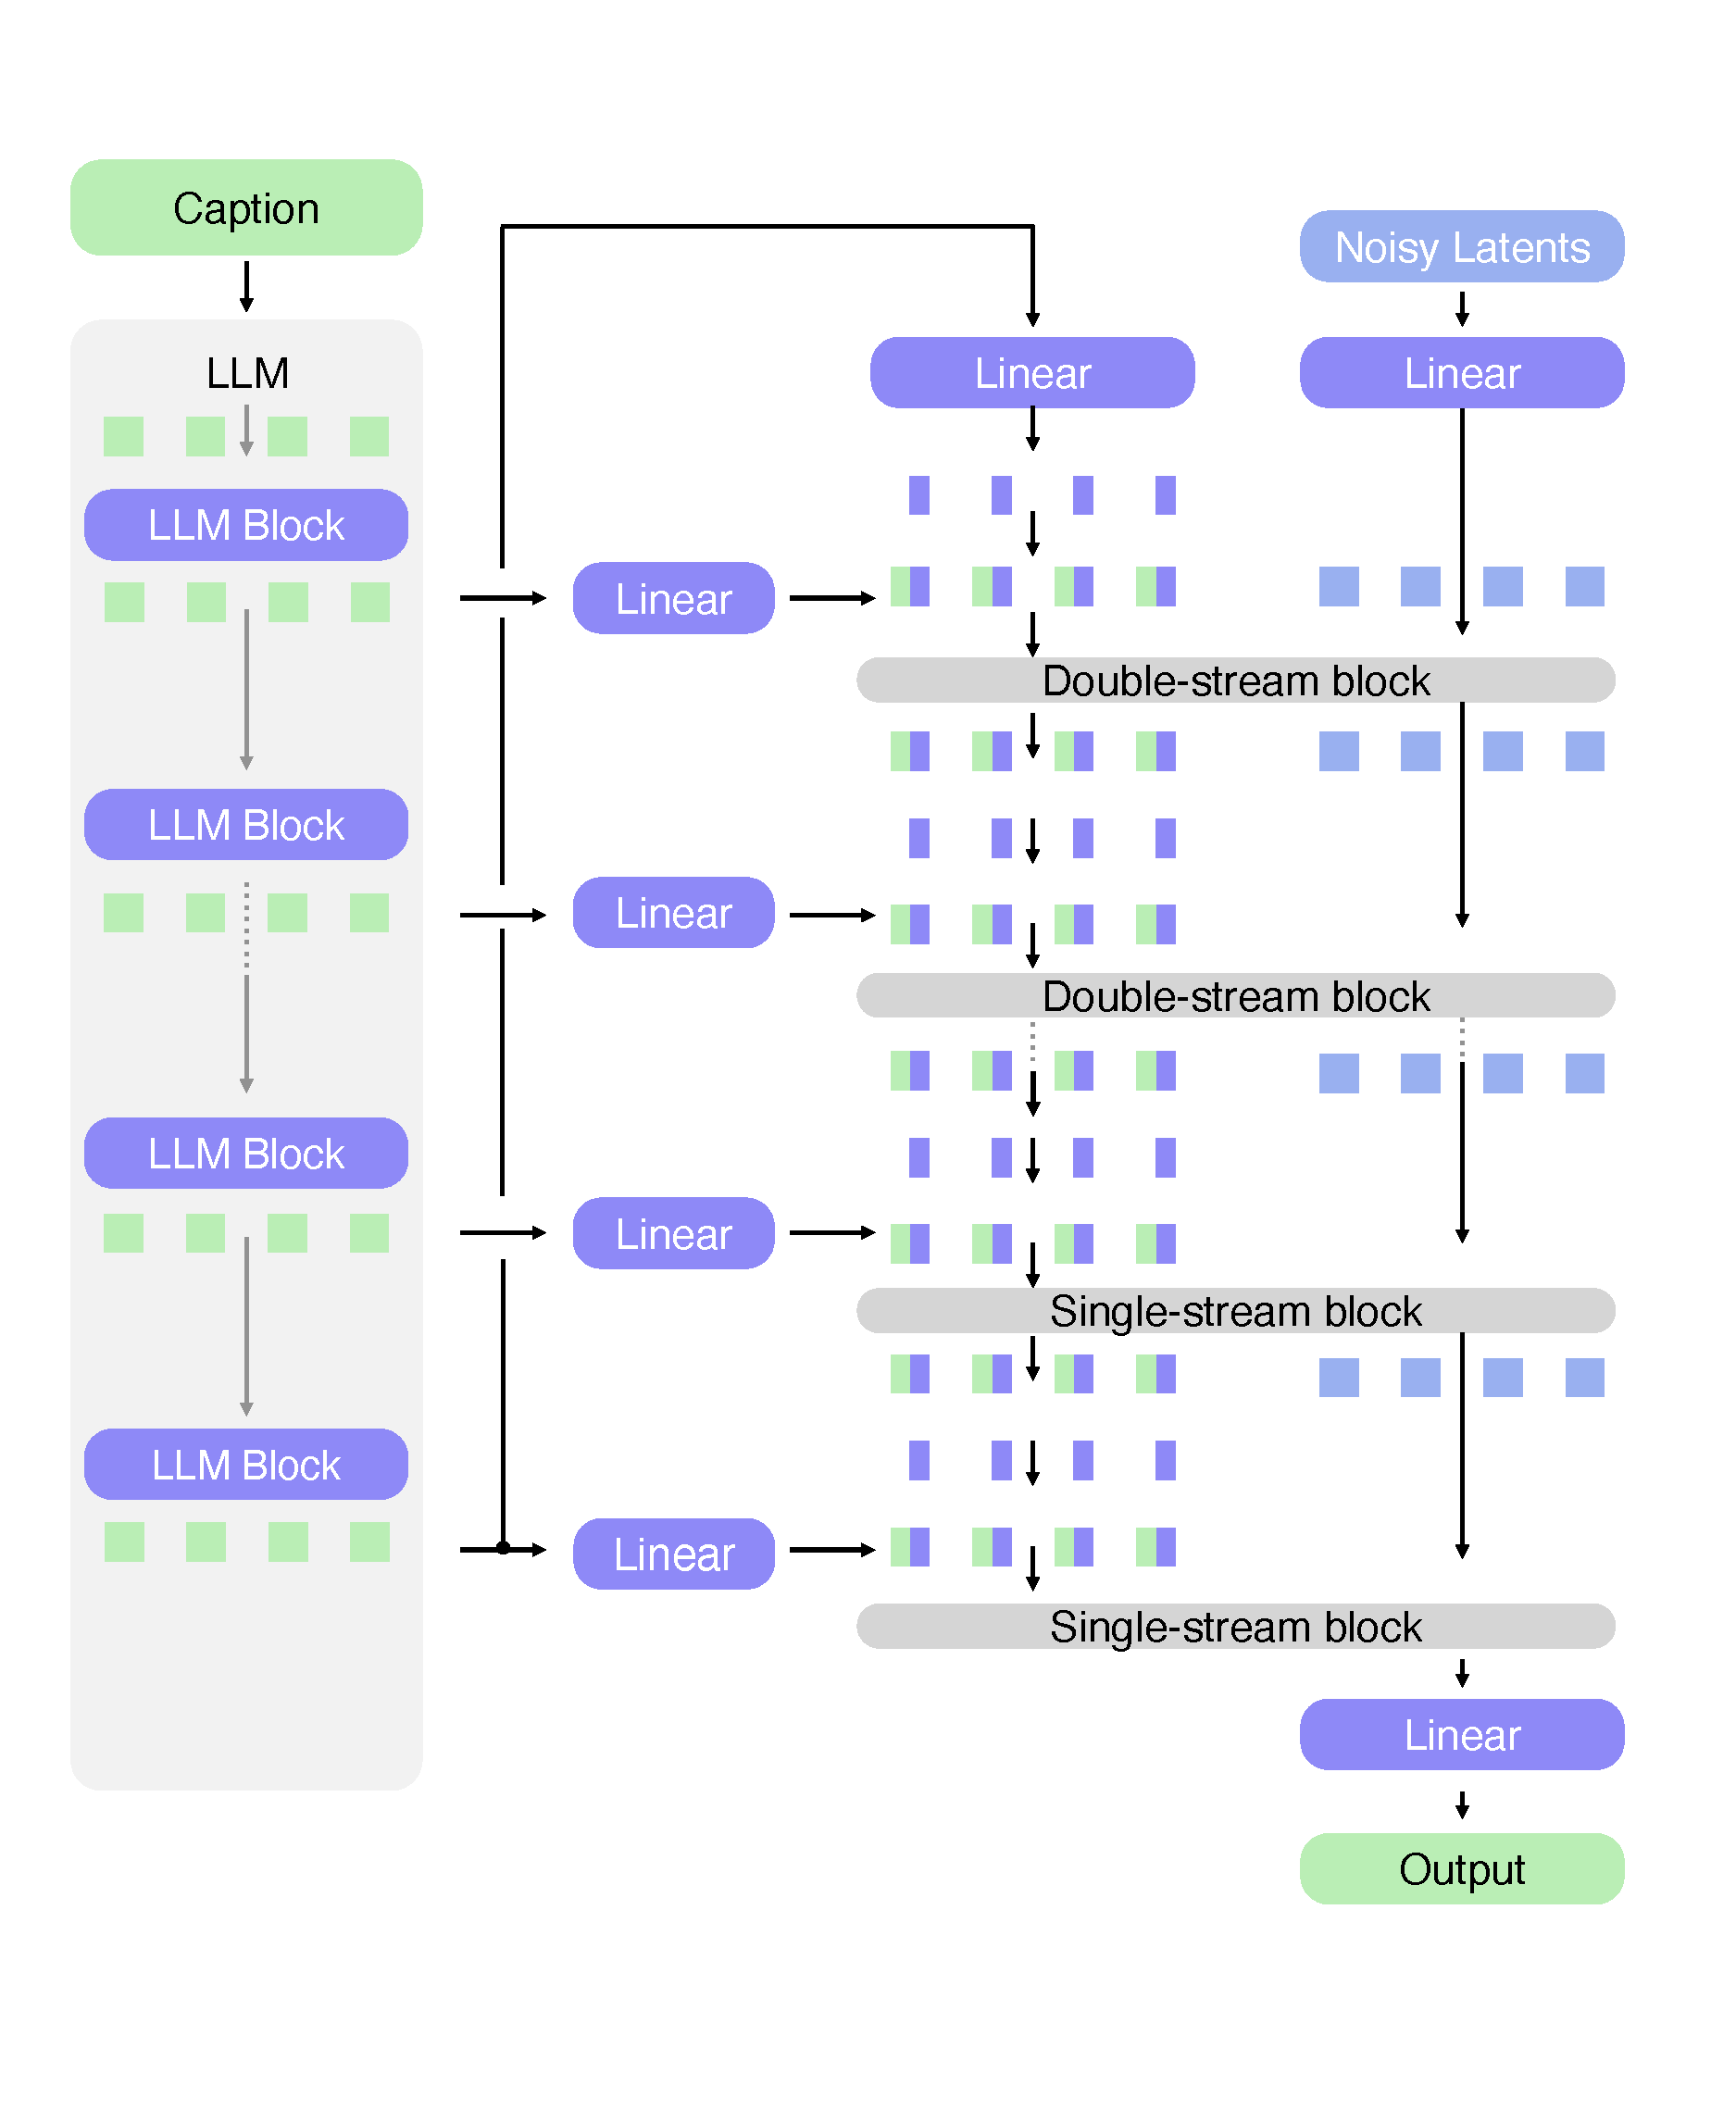
\includegraphics[width=\linewidth]{plots/model_figure2.pdf}
  \caption{\textbf{DimFusion architecture.} In each layer, the \textbf{\textcolor{textencoding}{text encoding}} is concatenated with the corresponding LLM \textbf{\textcolor{llmtokens}{hidden states}} along the embedding dimension. The resulting representation is then jointly processed with the \textbf{\textcolor{imagetokens}{noisy latents}} through bi-directional mixing in the Dual- and Single-stream blocks. After each block, the appended LLM hidden states are discarded, restoring the original text embedding dimension.}
  \label{fig:arch}
\end{figure}






We conducted an ablation study using a $1$B-parameter transformer with SmolLM3-3B as the LLM text encoder. 
As a baseline, we trained with the final layer of T5-XXL as the text encoding and no LLM fusion. 
Following HiDream~\cite{cai2025hidream}, we then evaluated \emph{TokenFusion}, where the text encoding is concatenated with the hidden states of the corresponding LLM block along the \emph{sequence} dimension. 
Finally, we assessed our proposed \emph{DimFusion}. 
All models were trained for 150k steps on 128 H200 GPUs with the same batch size (full training details appear in the appendix).
Figure~\ref{fig:dimfusion-merged} reports the training loss, FID and average time per step for these configurations. Both TokenFusion and DimFusion substantially outperform the T5-XXL baseline, confirming the value of LLM representations. 
Notably, DimFusion achieves a slightly better FID than TokenFusion while reducing the average step time from $0.8$ seconds to $0.5$ seconds, which corresponds to a $\sim$1.6× reduction in wall-clock time, demonstrating that DimFusion retains the advantages of deep LLM fusion while being more compute-efficient.




% \begin{figure}[h!]  % placement options: h, t, b, p
%     \centering
%     \resizebox{\linewidth}{!}{%
%     \includegraphics[width=0.7\textwidth]{plots/dimFusionComparison.png}
%     }
%     \resizebox{\linewidth}{!}{\includegraphics[width=0.7\textwidth]{plots/dimFusionDiff.png}
%     }
% \caption{\textbf{Training loss comparison for different text encoding architectures.} We compare T5 (baseline), SmolLM3-3B + TokenFusion, and SmolLM3-3B + DimFusion. \emph{Top:} Both fusion strategies outperform the T5 baseline, with DimFusion closely matching TokenFusion. \emph{Bottom:} Loss difference relative to TokenFusion, showing that DimFusion converges to the same value while requiring significantly lower computational cost.}

%     \label{fig:dimFusionComparison}
% \end{figure}


% Preamble (add if not already present):
% \usepackage{graphicx,array,booktabs}

\begin{figure}[t]
\centering

% ---------- TOP: FID table (inline, not a float) ----------
{\setlength{\tabcolsep}{8pt}\renewcommand{\arraystretch}{1.05}
\begin{tabular}{lcc}
\toprule
\textbf{Architecture} & \textbf{FID} ↓ & \textbf{Avg. Time per Step (sec)} ↓\\
\midrule
T5 & 36.46  & 1.28\\
TokenFusion & 15.90 & 0.8\\
DimFusion & \textbf{15.58} & \textbf{0.5}\\
\bottomrule
\end{tabular}
}

\vspace{6pt}

% ---------- BOTTOM: loss plots ----------
\resizebox{\linewidth}{!}{%
  \includegraphics[width=0.7\textwidth]{plots/dimFusionComparison.png}
}
\resizebox{\linewidth}{!}{%
  \includegraphics[width=0.7\textwidth]{plots/dimFusionDiff.png}
}

\vspace{-2pt}
\caption{\textbf{DimFusion vs. TokenFusion} \emph{Top:} FID on $30$K COCO-2014 val images~\cite{lin2014microsoft}: both fusion strategies (TokenFusion, DimFusion) substantially outperform T5, with \textbf{DimFusion} achieving the best FID while maintaining lower time per step. \emph{Middle:} Training loss comparison for T5 (baseline), SmolLM3-3B + TokenFusion, and SmolLM3-3B + DimFusion. Both fusion strategies outperform T5, with DimFusion closely matching TokenFusion. \emph{Bottom:} Loss difference relative to TokenFusion zoomed in, showing DimFusion converges to a similar value while requiring significantly lower computational cost.}
\label{fig:dimfusion-merged}
\end{figure}




% \input{tables/dimfusion_fid_compariosn}



\subsection{Evaluating Long Captions}
\label{sec:eval}



Most text-to-image models are evaluated through simple user-preference protocols, where participants are asked questions such as \textit{``which image do you prefer?''} given outputs from different models, e.g., ~\cite{esser2024scaling}. While this setting is effective for short prompts, it fails for \textbf{long structured captions} that often exceeding 1{,}000 words, since humans struggle to parse such detailed textual descriptions. Moreover, prior work has shown that preference-based evaluation tends to reward a characteristic \textit{``AI aesthetic''}, marked by over-saturated colors and excessive focus on central subjects, a phenomenon recently termed \textit{bakeyness}~\cite{batifol2025flux}. We argue that this evaluation paradigm hinders progress, as it incentivizes models to optimize for short prompts and average aesthetics, rather than expressive power and controllability.  


To overcome this, we propose \textbf{Text-as-a-Bottleneck Reconstruction (TaBR)}, a new evaluation protocol designed to suit long captions and generalize across domains and styles. Our key observation is that while humans find it difficult to digest long textual prompts, they can reliably compare complex images. TaBR leverages this asymmetry by introducing the image itself as the anchor for evaluation.  


Inspired by cycle-consistency principles~\cite{bahng2025cycle}, TaBR begins with a real image, which is first captioned. This caption is then provided as the sole input to the generator, producing a reconstructed image. Finally, we compare the reconstructed outputs to the original. In practice, we generate two candidate reconstructions and ask annotators: \textit{``which image is more similar to the original?''} Unlike standard preference scoring, user judgments in TaBR are guided by the original image, which conveys far richer detail than a short textual description. By controlling the set of real images used in evaluation, we prevent judgments from collapsing into personal taste and instead obtain a direct measure of the model’s expressive power. An example appears in Figure~\ref{fig:tabr}: our model is the only one that preserves the pose in the second and bottom rows, demonstrating superior controllability using text alone. Quantitative results are reported in Section~\ref{sec:Quantitative_Results}.

% \ekc{Are we going to provide a dataset for this evaluation benchmark?} \ron{This is a really good - we should think about it}

% Quantitative results are provided in ?. As can be seen in Fig.? our evaluation highlights our model's ability to follow long and detailed descriptions... \ekc{This is not necessary here, right? We can just give a reference to the experiment section.}




% Preamble: \usepackage{graphicx,array}
\setlength{\tabcolsep}{0.5pt}
\renewcommand{\arraystretch}{1.0}

\begin{figure}[t]
\centering
\newcommand{\imgw}{0.24\linewidth} % 4 images × 0.24 = 0.96 (safe)
\begin{tabular}{@{}cccc@{}}
  % Header
  % \multicolumn{4}{@{}l@{}}{{\scriptsize\textbf{Structured edits (disentanglement)}}} \\[-1pt]

  % Images (row)
  \includegraphics[width=\imgw]{Figures/tabr/images/1.jpg} &
  \includegraphics[width=\imgw]{Figures/tabr/images/1_flux.jpg} &
  \includegraphics[width=\imgw]{Figures/tabr/images/1_qwen.jpg} &
  \includegraphics[width=\imgw]{Figures/tabr/images/1_bria_new.jpg}
  \\[-2pt]

    % Images (row)
  \includegraphics[width=\imgw]{Figures/tabr/images/17.jpg} &
  \includegraphics[width=\imgw]{Figures/tabr/images/17_flux.jpg} &
  \includegraphics[width=\imgw]{Figures/tabr/images/17_qwen.jpg} &
  \includegraphics[width=\imgw]{Figures/tabr/images/17_bria.jpg}
  \\%[-2pt]

    % Images (row)
  \includegraphics[width=\imgw]{Figures/tabr/images/22.jpg} &
  \includegraphics[width=\imgw]{Figures/tabr/images/22_flux.jpg} &
  \includegraphics[width=\imgw]{Figures/tabr/images/22_qwen.jpg} &
  \includegraphics[width=\imgw]{Figures/tabr/images/22_bria_new.jpg}
  \\%[-2pt]

    % Images (row)
  \includegraphics[width=\imgw]{Figures/tabr/images/52.jpg} &
  \includegraphics[width=\imgw]{Figures/tabr/images/52_flux.jpg} &
  \includegraphics[width=\imgw]{Figures/tabr/images/52_qwen.jpg} &
  \includegraphics[width=\imgw]{Figures/tabr/images/52_1024_1024.jpg}
  \\%[-2pt]

  % Wrapped labels under each image (row)
  \parbox{\imgw}{\scriptsize\centering \textbf{Original}} &
  \parbox{\imgw}{\scriptsize\centering \textbf{Flux}} &
  \parbox{\imgw}{\scriptsize\centering \textbf{Qwen-Image}} &
  \parbox{\imgw}{\scriptsize\centering \textbf{\modelname{} (Ours)}}
  \\
\end{tabular}

\vspace{-3pt}
\caption{\textbf{Text-as-a-Bottleneck Reconstruction (TaBR).} We caption the original image and use the resulting text as a bottleneck input to the generator, producing a reconstructed image. This evaluation allows humans to assess a model’s expressive power objectively without reading extremely long captions. As shown, our model achieves noticeably higher similarity to the original image.}
\label{fig:tabr}
\end{figure}

\begin{table}[t]
  \centering
  \footnotesize
  \begin{tabular}{cccccc}
    \toprule
    \textbf{\makecell{Dual-stream \\ Blocks}} &
    \textbf{\makecell{Single-stream \\ Blocks}} &    
    \textbf{\makecell{FFN \\ Dimension}} &
    \textbf{\makecell{Attention \\ Heads}} &
    \textbf{\makecell{Head dim}} &
    $\left(d_t, d_h, d_w\right)$ \\
    \midrule
    8 & 38 & 12288 & 24 & 128 & $(16,\,56,\,56)$ \\
    \bottomrule
  \end{tabular}
  \caption{\textbf{\modelname{} transformer architecture.}}
  \label{tab:model_arch}
\end{table}




\subsection{Large Scale Training}\label{sec:training}


\begin{table*}[!t]\centering
\renewcommand{\arraystretch}{1.7} 
\setlength{\tabcolsep}{3pt}

\centering
\begin{adjustbox}{width=\textwidth}
\begin{tabular}{l|ccc|ccc|ccc|ccc|ccc|ccc|ccc}
\toprule
\multirow{2}{*}{\textbf{Model}}
  & \multicolumn{3}{c|}{\textbf{Imagination}}
  & \multicolumn{3}{c|}{\textbf{Text rendering}}
  & \multicolumn{3}{c|}{\textbf{Style}}
  & \multicolumn{3}{c|}{\textbf{Affection}}
  & \multicolumn{3}{c|}{\textbf{Composition}}
  & \multicolumn{3}{c|}{\textbf{Long text}}
  & \multicolumn{3}{c}{\textbf{Overall}} \\

\cmidrule(lr){2-22}

% ── 2nd header row ───────────────────────────────────────────────────────────
  & Ali. & Aes.& Avg.
  & Ali. & Aes.& Avg.   
  & Ali. & Aes.& Avg.     
  & Ali. & Aes.& Avg.        
  & Ali. & Aes.& Avg.     
  & Ali. & Aes.& Avg.     
  & Ali. & Aes.& Avg.     
  \\

\midrule


SD3.5-Large~\citep{SD35} & 75.4 & 75.2 & 75.3 & 56.1 & 68.3 & 62.2 & 78.3 & 81.0 & 79.7 & 87.7 & 86.4 & 87.0 & 86.6 & 83.1 & 84.9 & 67.8 & 59.2 & 63.5 & 78.8 & 77.6 & 78.2\\

FLUX.1-dev~\citep{flux2024} & 65.4 & 71.8 & 68.6 & 57.4 & 63.5 & 60.4 & 71.4 & 80.4 & 75.9 & 88.5 & \underline{89.3} & 88.9 & 89.4 & 85.4 & 87.4 & 73.3 & 66.8 & 70.1 & 77.0 & 78.7 & 77.8\\

FLUX.1-Krea-dev~\citep{fluxkrea} & 71.4 & 73.3 & 72.4 & 52.6 & 62.6 & 57.6 & 79.4 & 84.3 & 81.9 & 86.8 & \textbf{89.6} & 88.2 & 90.0 & 86.6 & 88.3 & 77.1 & 65.9 & 71.5 & 79.7 & 79.7 & 79.7\\

HiDream-I1-Full~\citep{cai2025hidream} & 74.1 & 74.4 & 74.2 & 64.8 & 72.2 & 68.5 & 79.3 & \underline{88.8} & 84.1 & \underline{90.8} & 87.8 & 89.3 & 90.3 & \underline{86.7} & 88.5 & 64.0 & 53.7 & 58.8 & 80.0 & 79.1 & 79.5\\

Qwen-Image~\citep{wu2025qwenimagetechnicalreport} & 79.4 & \underline{81.0} & 80.2 & \textbf{76.1} & \underline{76.5} & \textbf{76.3} & 79.9 & 86.4 & 83.1 & 85.8 & 87.2 & 86.5 & \textbf{94.2} & 84.4 & \underline{89.3} & 82.4 & 65.9 & 74.1 & 84.1 & 81.5 & 82.8\\

% FireFly~\citep{} & \textbf{92.4} & \underline{84.8} & \textbf{88.6} & \underline{87.0} & \underline{81.3} & \underline{84.2} & \underline{65.2} & \underline{74.1} & \underline{69.7} & \underline{90.5} & \underline{90.8} & \underline{90.7} & \textbf{96.0} & 88.2 & \textbf{92.1} & 92.5 & \underline{88.5} & \underline{90.5} & \textbf{85.9} & \textbf{76.2} & \textbf{81.1} & \textbf{87.1} & \underline{83.4} & \underline{85.3} \\

\midrule
Gemini2.5-Flash-Image~\citep{comanici2025gemini} & \textbf{91.4} & \textbf{86.9} & \textbf{89.1} & \underline{71.3} & \textbf{78.7} & \underline{75.0} & \textbf{89.9} & \textbf{90.6} & \textbf{90.2} & \textbf{97.4} & 88.4 & \textbf{92.9} & \underline{92.6} & \textbf{90.3} & \textbf{91.5} & \textbf{88.1} & \textbf{81.4} & \textbf{84.8} & \textbf{91.2} & \textbf{87.3} & \textbf{89.3}\\

% GPT-Image-1 [High]~\citep{gptimage} & \underline{86.2} & \textbf{86.6} & \underline{86.4} & \textbf{90.0} & \textbf{86.3} & \textbf{88.2} & \textbf{68.8} & \textbf{80.1} & \textbf{74.5} & \textbf{92.8} & \textbf{93.3} & \textbf{93.1} & 90.7 & \underline{90.9} & \underline{90.8} & \textbf{96.2} & \textbf{89.4} & \textbf{92.8} & \underline{83.8} & \underline{72.8} & \underline{78.3} & \underline{86.9} & \textbf{85.6} & \textbf{86.3} \\
\midrule
% GAIA (v1) & 87.9 & 74.2 & 81.1 & 59.1 & 64.3 & 61.7 & 78.9 & 83.3 & 81.1 & 91.6 & 73.7 & 82.7 & 87.6 & 74.3 & 81.0 & 75.2 & 52.9 & 64.0 & 83.3 & 70.6 & 77.0\\
% GAIA-previous (Ours) & \textbf{93.2} & 78.1 & \underline{85.6} & 66.1 & 65.7 & 65.9 & \underline{85.4} & 87.8 & \underline{86.6} & \underline{94.2} & 83.8 & 89.0 & 91.2 & 80.1 & 85.7 & \underline{83.7} & 63.5 & 73.6 & \underline{89.0} & 78.6 & \underline{83.8}\\

\modelname{} (Ours) & \underline{90.5} & 77.6 & \underline{84.0} & 66.5 & 72.2 & 69.3 & \underline{86.9} & 86.9 & \underline{86.9} & 90.3 & 88.4 & \underline{89.4} & 91.1 & 85.5 & 88.3 & \underline{83.2} & \underline{72.1} & \underline{77.7} & \underline{87.8} & \underline{82.1} & \underline{84.9}\\
\modelname{} open-VLM & 88.5 & 76.2 & 82.3 & 65.2 & 68.7 & 67.0 & 85.1 & 88.5 & 86.8 & 89.5 & 87.3 & 88.4 & 90.1 & 85.1 & 87.6 & 82.1 & 67.5 & 74.8 & 86.4 & 80.9 & 83.6\\
\bottomrule

\end{tabular}
\end{adjustbox}
\caption{\textbf{Quantitative results on PRISM-Bench-licensed:} a licensed variant of PRISM~\cite{fang2025flux}. We report alignment (Ali.), aesthetics (Aes.), and average (Avg.)  across categories. Best results are in \textbf{bold}; second best are \underline{underlined}. \modelname{} outperforms all open-source baselines.}
\label{tab:prism}

\end{table*}
\begin{table*}
%\renewcommand{\arraystretch}{1.7} 
\setlength{\tabcolsep}{3pt}
  \centering
  \begin{adjustbox}{width=\textwidth}
  \begin{tabular}{lcccccccc}
    \toprule
    \textbf{Model} & \textbf{Size (Parameters)} & \textbf{Single object} & \textbf{Two object} & \textbf{Counting} & \textbf{Colors} & \textbf{Position} & \textbf{Color attribution} & \textbf{Overall} \\    
    \midrule
    SD3.5-Large~\citep{SD35} & 8B & \textbf{1.00} & 0.91 & \underline{0.79} & 0.81 & 0.23 & 0.54 & 0.71 \\
    FLUX.1-dev~\citep{flux2024} & 12B & \underline{0.99} & 0.80 & 0.75 & 0.77 & 0.19 & 0.49 & 0.66 \\
    FLUX.1-Krea-dev~\citep{fluxkrea} & 12B & \underline{0.99} & 0.91 & 0.70 & 0.88 & 0.31 & 0.69 & 0.75 \\
    HiDream-I1-Full~\citep{cai2025hidream} & 17B & \textbf{1.00} & \textbf{0.98} & \underline{0.79} & \textbf{0.91} & 0.60 & \underline{0.72} & 0.83 \\
    Qwen-Image~\citep{wu2025qwenimagetechnicalreport} & 20B & \underline{0.99} & \underline{0.94} & \textbf{0.91} & 0.87 & \underline{0.77} & \textbf{0.75} & \textbf{0.87} \\
    \midrule
    % GAIA(v1) & 0.98 & 0.92 & 0.66 & 0.87 & 0.78 & 0.52 & 0.79 \\
    \modelname{} (Ours) & 8B & \textbf{1.00} & 0.88 & \underline{0.79} & \underline{0.90} & \textbf{0.80} & 0.71 & \underline{0.85} \\
    \bottomrule
  \end{tabular}
  \end{adjustbox}
\caption{\textbf{Quantitative results on the GenEval benchmark.} Best results are shown in \textbf{bold}, and second best are \underline{underlined}. Unlike PRISM-Bench, GenEval focuses on relatively short captions. Accordingly, our model \modelname{} achieves comparable performance to other open-source models despite using fewer parameters.}


  \label{tab:geneval}
\end{table*}


We demonstrate the effectiveness of our contributions through \emph{\modelname{}}, a large-scale text-to-image model with $8$B parameters trained entirely on long structured captions. 
\modelname{} adopts the DimFusion architecture introduced in Section~\ref{sec:dimfusion}, using \emph{SmolLM3-3B}~\cite{bakouch2025smollm3} as the fused LLM backbone. The model operates in the latent space~\cite{rombach2022high} with the Wan~2.2 VAE~\cite{wan2025wan} and a patch size of $1$. 
Additional hyperparameters are summarized in Table~\ref{tab:model_arch}.


Training is performed on $120$M licensed image–caption pairs, where captions are long, structured JSONs generated by \emph{Gemini~2.5}~\cite{comanici2025gemini}, as described in Section~\ref{sec:captions}. We employ progressive training, starting at low resolutions and gradually increasing throughout. We initialize with REPA~\cite{yu2024representation} using a coefficient of $0.1$ for the first $300$K low-resolution steps, followed by mixed-resolution training. After pretraining, we apply aesthetic finetuning with $3{,}000$ hand-picked images, then DPO training~\cite{wallace2024diffusion} with dynamic beta~\cite{liu2025improving} to improve text rendering. Additional implementation details, including optimization and data distribution, are provided in the Appendix.

